\documentclass{sigplanconf}
%\documentclass[preprint]{sigplanconf}

\usepackage{amsmath}
\usepackage{graphicx}
\usepackage{url}

\def\META#1{\textit{${\cal MET\!\!A}$#1}}
\def\TODO#1{\texttt{\bf {TODO:} #1}}

\begin{document}

\conferenceinfo{VEE 2008}{March 5--7 2008, Seattle, USA.}
\copyrightyear{2007}
%\copyrightdata{[to be supplied]} 

\preprintfooter{DRAFT $\null$Revision: 1.5 $\null$}

\title{Magrathea: Enabling New Applications Using Cluster Virtualization}

\authorinfo
    {Ji\v{r}\'\i{} Denemark}
{%
Cesnet~z.\,s.\,p.\,o.,\\
Zikova~4, 160~00 Praha 6,\\
Czech Republic\\
and\\
Faculty of Informatics, \\
Masaryk University,\\
Botanick\'a 68a, 602~00 Brno,\\
Czech Republic
}
    {jirka@ics.muni.cz}

\authorinfo
    {Miroslav Ruda}
{%
Cesnet~z.\,s.\,p.\,o.,\\
Zikova~4, 160~00 Praha 6,\\
Czech Republic\\
and\\
Institute of Computer Science,\\
Masaryk University,\\
Botanick\'a 68a, 602~00 Brno,\\
Czech Republic}
    {ruda@ics.muni.cz}


\maketitle

\begin{abstract}

Traditional batch scheduling systems used for high performance computing
started to limit people in applications which they are able to run on such
systems. Nowadays people often require more than submitting a job to a queue
and waiting until scheduling system decides to run it. For example, resource
owners may provide their resources for jobs of other users, but may require
higher priority for accessing them. Another class of applications require
interactive access to computing resources when users dynamically influence the
computation which may result in a sudden need for more resources required to
finish the task. Such requirements may be satisfied with the help of virtual
machines deployed on computational machines. In this paper, we provide a
description of a system called Magrathea, which we have created to allow job
scheduling system to deal with several virtual machines (VMs) running on a
single computer and to submit jobs into those VMs. Virtual machines may
provide different execution environments for user's jobs with different
allocation of resources. Magrathea manages resources given to each virtual
machine so that several VMs are allowed to share a single node and its
resources according to site requirements. It is designed to be general and
flexible with a minimum set of modifications required for specific batch
system. Virtual machines running on a single node are managed by a dedicated
daemon on the same node. This way different resources managed by a single
batch scheduling system may provide different access policies and sharing of
resources among virtual machines. In a more complicated schema, each virtual
machine on the same node can even be managed by different scheduling system.

\end{abstract}

%\category{CR-number}{subcategory}{third-level}

\terms batch system, virtual machine monitor, virtual machine
\keywords cluster virtualization, grid computing, preemption, heterogeneous
    environment


\section{Introduction}

Systems for high performance computing as well as current grids usually use
some kind of batch scheduling system to schedule users' jobs on computing
resources. As batch processing systems cannot usually guarantee executing a
job in a particular time, batch processing is great for long computations when
users do not set tight deadlines for them. Nowadays, there are more and more
applications which require data to be processed as soon as it is ready.
Moreover, some applications require interactivity. For example, data obtained
from a microscope has to be processed and analyzed by a user who decides which
parts of the image are important and more detailed images should be taken of
them. All this has to be done interactively within a few minutes before the
material under the microscope is destroyed. Some resource owners may allow
jobs of other users running on their resources, but they may also require
higher priority for their jobs (including immediate access) to those
resources. For such scenarios, where people require more than just submitting
a job to a queue and waiting until scheduling system decides to run it, pure
batch processing is not sufficient and it has to be extended or replaced with
a more flexible system.

Of course, users' requirements can be to some extent fulfilled by playing with
different queues, job priorities, advance reservations and so on. However,
without the ability to preempt running jobs a scheduling system can hardly
guarantee immediate execution of interactive jobs. While batch scheduling
systems may provide support for job preemption, it is limited to what
operating systems running on computing machines support. Usually, job
preemption is achieved by completely suspending a process or reducing its
priority possibly combined with setting additional limits. But it is hard to
enforce such limits and ensure a new job is not slowed down by a preempted
job---either directly or indirectly through an operating system by, e.\,g.,
swapping. Complete suspend might seem to be a good solution but it has serious
impact on parallel jobs or processes communicating over a network.

With virtual machine technology, which provides strong isolation of processes
running within different virtual machines, better preemption without
unpredictable performance losses can be achieved by applying limits and
resource restrictions on a virtual machine as a whole instead of applying them
on just a single process.

Virtual machines are also useful when some computing resources have to be
shared among different projects. Each project usually requires its own
installation of operating system and applications tailored to specific
requirements of the project. Moreover, different projects may require
different middleware systems to be used for accessing resources and scheduling
jobs. These systems have to be able to cooperate when accessing shared
resources.

We have created a system called Magrathea to allow job scheduling system to
deal with several virtual machines running on a single computer and to submit
jobs into those VMs. Furthermore, Magrathea is designed to be independent on
a batch system and virtual machine monitors used on computational nodes.

Magrathea is deployed in production environment on computational nodes of
\META{Center}\footnote{http://meta.cesnet.cz/}, which provides a computational
infrastructure for various groups of users with specific requirements and its
resources are also provided for European grid infrastructure
EGEE\footnote{http://www.eu-egee.org/}. The primary motivation for deploying
virtual machines was integrating \META{Center} resources into EGEE
infrastructure as they require different software configuration on
computational resources. However, using Magrathea, we can provide users with
much more then just the possibility to run their jobs in two different
environments.

In the following section we describe some related work,
Section~\ref{sec:magrathea} provides detailed description of Magrathea and its
implementation. In Section~\ref{sec:deployment} we talk about experiences with
a deployment of Magrathea on our production cluster. Finally, we conclude the
paper and outline enhancements to Magrathea planned for the near future.


\section{Related Work}

Scheduling which can guarantee deadlines may be achieved using advance
reservations. Various resource management systems support advance reservation
of resources (e.\,g., PBS~\cite{pbs}, Maui~\cite{maui}, LSF~\cite{lsf},
CCS~\cite{ccs}). While this technique is useful for co-allocation of
resources, advance reservation can also degrade quality of schedule (waiting
time of queued jobs or resource utilization~\cite{smith}). According
to~\cite{singh} (and a survey cited in that paper), advance reservations are
still not provided by regular sites and even if they are provided, human
intervention may be required for getting such reservations.

Problem of job preemption is also well-known for resource management systems
which support ``cycle stealing'', such as Condor~\cite{condor}. In such
environment, a job is running only when resource is not used by owner and
resource must be given back to resource owner immediately when requested. In
Condor, the ability to preempt jobs is achieved by recompilation of
applications, which substitutes all I/O system calls with variants supporting
either checkpointing or remote I/O.

As virtualization has recently become very popular in high performance
computing, several projects have appeared trying to deal with virtual machines
on worker nodes of computational clusters. As for the original motivation,
probably the closest project to ours was started by physicists in
Karlsruhe~\cite{karlsruhe}. In parallel to our effort, they observed the same
potential in deploying virtual machines for sharing resources among several
groups of users, each requiring different computing environment. Although the
initial motivation was the same, their approach is different. They decided to
create a separate daemon which actually manages all jobs, resources, and
virtual machines. When a new VM is created for a job on the top of a queue,
the VM is made available for a batch queuing system, which submits the job
into it. This approach is very interesting but quite difficult to implement as
it ends up with reimplementing most parts of batch queuing system within the
daemon.

Another interesting project aims to provide dynamic virtual
clustering~\cite{dvc} (DVC) using Xen virtual machine monitor, Moab workload
manager and TORQUE resource manager. Working in cooperation with Moab
developers the authors of DVC managed to provide transparent creation of
clusters of virtual machines. Virtual clusters are also allowed to span
multiple physical clusters by borrowing required resources from resource
managers of the other clusters. However, as it was heavily integrated with
Moab, DVC is closely bound to the Moab/TORQUE combination. On the other hand,
our solution---Magrathea---is made much more general with respect to required
scheduling system and virtual machine monitor. DVC also includes system image
management so that each virtual machine is started from an image required by a
job for which the virtual machine is being created. As virtual machines in DVC
are created and stopped dynamically, a lot of work had to be done to assure
correct registration of new resources at all relevant parts of the system.
Likewise, destroyed virtual machines must be removed from a pool of resources
available for job scheduler. As Magrathea uses virtual machines which are not
created and destroyed dynamically, we do not need to modify batch system to be
able to cope with frequent changes of available computational resources.

Magrathea does not cover management of system images for virtual machines and
we do not expect a batch system to do this job either. Instead, existing
systems, such as Virtual Workspaces~\cite{workspaces} or
In-VIGO~\cite{invigo}, can be used for that purpose. This separation not only
simplifies the design of Magrathea but also makes sharing resources among
several batch systems easier as it reduces the number of changes to those
batch systems.


\section{Magrathea}
\label{sec:magrathea}

The key features of Magrathea are its independence on VMM and a batch system
and its flexibility in usage scenarios for which it can be used. It provides a
transparent interface between a job scheduling system and VMM used on each
machine.

\subsection{Architecture}

The whole Magrathea system consists of three building blocks:
\begin{itemize}
\item status cache,
\item master daemons,
\item slave daemons.
\end{itemize}

In addition, Magrathea cooperates with a virtual machine monitor (VMM) and
a batch queuing system. The architecture of Magrathea and interactions with
other parts of a whole computational environment is depicted in
Figure~\ref{fig:architecture}.

\begin{figure}[tb]
    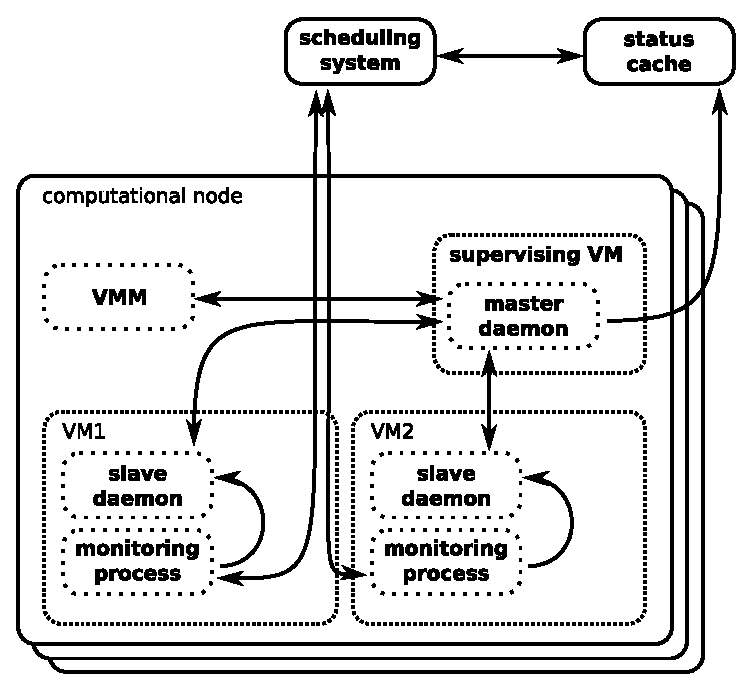
\includegraphics[width=\columnwidth]{architecture}
    \caption{The architecture of Magrathea (scheduling system and monitoring
        processes are parts of a batch system).}
    \label{fig:architecture}
\end{figure}

\textit{Status cache} stores status data about all virtual worker nodes so
that a batch scheduling system does not have to contact each node to check its
current status before making a decision where to execute a job. This part is
not required when a scheduling system is able to get status information
directly from computational nodes. However, the status cache is a more
scalable solution.

\textit{Master daemon} runs on each real machine and manages all virtual
worker nodes running on the same machine and stores their current status at
the status cache. The status cache is updated whenever the status is changed
and even when no change occurs within a predefined time period.

\textit{Slave daemon} runs on each virtual worker node and asks its master
daemon for permission to start a new job, informs the master about finished
jobs and behaves according to commands received from the master.

Basic interactions among all parts of Magrathea and a batch scheduling system
for a single job are as follows, interactions between Magrathea and the rest
of the system will be further described in the following section. When a job
comes to the batch queuing system, the scheduler gets a list of all nodes (a
mixture of virtual and real nodes is allowed). Then, for each virtual node,
the scheduler asks the status cache for the current status of that virtual
node. Having fetched all required information, the scheduler makes a decision
which node (or a set of nodes in case of parallel job) is the best one to be
used for the job as usual but it also takes into account information from the
status cache. Just before executing the job, the slave daemon running on each
of the selected virtual nodes is contacted by a monitoring process of the
batch system to check with the master daemon whether the job can really be
executed. If it is allowed to be executed, the master daemon changes the
status of its virtual nodes, performs some VMM specific actions and updates
the status cache. When a job is finished, the monitoring process of the batch
system contacts the particular slave daemon, which---this time
asynchronously---tells it to its master daemon. Then the master changes the
status, executes VMM specific actions, and updates the status cache.

\subsection{Implementation}

In current implementation of Magrathea, all virtual machines---either running
a job or being idle---are always running although with different resource
allocation. This way, a batch system may think of all virtual machines as
usual and may keep monitoring them. Also automatic upgrades, remote
configuration and other management activities do not have to cope with virtual
machines which are only occasionally running. However, when idle virtual
machines are required to be completely suspended, a batch system can be
modified to honor information from a status cache and to exclude suspended
virtual machines from its monitoring process.

Magrathea is independent on both VMM and batch scheduling system and it can
even be used by several batch systems at the same time. When, for example,
several batch systems share a real machine providing different virtual
machines for different systems, Magrathea can be used to make those batch
systems cooperate. Naturally, all parts bound to a particular VMM are isolated
on a physical machine, which enables the whole system to transparently use
machines with various virtual machine monitors.

Master daemon provides an interface to a VMM so that specific actions can be
performed to activate and deactivate virtual machines, change resources they
are allowed to use and so on. The interface is generic and completely
different code can be executed for different VMMs. Another interface to a VMM
is used to match slave daemons with virtual machines they are running on and
to detect virtual machines which do not exist any more. In the beginning we
have used Xen virtual machine monitor~\cite{xen} for running virtual machines.
However, because Xen does not allow for sharing physical memory among virtual
machines, the overhead of VMs which are not running any job is quite large and
grows linearly with increasing number of VMs (i.\,e., distinct computational
environments). For some cases, this overhead might be reduced by using
different VMM, such as VServer~\cite{vserver}, which allows for easy sharing
of memory among virtual machines. VServer or similar VMM may also be useful
for accessing specific hardware devices in a more efficient manner. Current
version of Magrathea supports both Xen and VServer.

Another interface is used for communication between Magrathea and batch
scheduling system on each worker node. Hooks executed by batch scheduling
systems when a job is started or stopped are used to communicate with a master
daemon through a particular slave daemon. This way Magrathea is informed about
jobs coming from a scheduling system. Central services, such as scheduler or
resource manager, use only information provided by the status cache for
deciding what resources are usable for executing new jobs.


\subsection{Use-cases}

We have decided to implement and deploy Magrathea on our computational
machines incrementally in several steps, so that we can start providing new
services for users without reduced reliability and long outages of available
resources. As master daemons are the only part of Magrathea which enforces how
jobs are allowed to be submitted to particular virtual machines, each usage
scenario requires only the logic in the master daemon and, for more
complicated scenarios, the slave daemon to be changed. This makes the whole
system very flexible and each real machine can even behave in a different way,
according to its purpose.

\subsubsection{Statically Deployed Virtual Machines}

The first step to deploy Magrathea was rather simple. Each VM-enabled
computational machine runs two distinct virtual machines, one for EGEE jobs
and the other one with \META{Center} environment. A virtual machine can be in
either \textit{free}, \textit{running}, or \textit{occupied} state, which
means that it is able to accept a job, it is currently running a job or it is
not allowed to accept any job, respectively. At most one of the machines can
be running a job, the other VM is occupied until the job is finished.
Figure~\ref{fig:twoVMs} shows states of two virtual machines and transitions
between them. As only one virtual machine can be running at a time, it is
provided with almost all memory and CPU power of the underlying physical host.
This way physical resources are dynamically provided for EGEE and
\META{Center} users according to current needs. 

\begin{figure}[tb]
    
\includegraphics[width=\columnwidth]{twoVMs}
    \caption{States and transitions between them for statically deployed
        virtual machines.}
    \label{fig:twoVMs}
\end{figure}

The reason why the virtual machine which is running a job is not given all the
memory and CPU power is that all VMs (regardless of whether they are running
jobs or not) have to be able to answer requests from PBS server. Thus, all VMs
must be running, although with low priority, and cannot be just suspended and
woken up when a job comes. Some memory and CPU power is also consumed by
supervising virtual machine.

\subsubsection{Preemption of Virtual Machines}

The second step in deploying virtual machines was to enable preemption of jobs
running inside virtual machines. This is especially useful to satisfy the
increasing demands for more predictable behavior of a scheduling system
required by new interactive or real-time applications. Preemption also helps
the system to immediately provide resources for people who paid for them.

In this case, two separate virtual machines with the same environment are
running on each worker node. One of them is used for normal jobs and the other
one for high-priority jobs which are allowed to preempt normal jobs. From the
other side, the virtual machine used for normal jobs can be seen as it is used
for backfilling when there is no high-priority job running. The preemption
adds three more states to those mentioned in the previous section:
\textit{occupied-would-preempt}, \textit{running-preemptible} and
\textit{preempted}.

As we consider some jobs as non-preemptible, two different states are used for
a virtual machine running a job. When non-preemptible job is running (running
state) all other virtual machines are in state occupied and no job can be
submitted into them. When, on the other hand, a preemptible job is running
within a normal virtual machine, a high-priority one is in
occupied-would-preempt state so that scheduler can distinguish between
machines which are really free and machines which can be used for submitting
jobs but doing so would preempt already running jobs. The third new
state---preempted---is the state of a virtual machine which was running a job
when another job was submitted into a high-priority VM. States and actions
which result in transitions between states are shown in
Figure~\ref{fig:preemption}. Access to both high-priority and normal VMs is
completely under control of the scheduling system. Magrathea just ensures
proper resource allocations for each virtual machine. However, to help the
scheduler with making better decisions, the status cache provides number of
seconds each virtual machine was preempted, which may be used to avoid
repeated preemption of the same virtual machine.

\begin{figure}[tb]
    
\includegraphics[width=\columnwidth]{preemption}
    \caption{States and transitions between them for preemption of virtual
        machines.}
    \label{fig:preemption}
\end{figure}

As VM preemption can be combined with the previous scenario, where virtual
machines were used for providing different execution environments, more than
one high-priority VM may be running on a single physical machine. In such a
case, all high-priority VMs are marked as free or occupied-would-preempt as
long as none of them is running any job. When a job which is allowed to
preempt other jobs arrives to a high-priority VM, the state of the virtual
machine which has been marked as running-preemptible (if there is such a VM)
is changed to preempted. States of other high-priority VMs are turned to
occupied so that no other job is allowed to be submitted on the particular
worker node. When the privileged job finishes, the preempted virtual machine
is returned back into running-preemptible and all high-priority VMs are marked
as occupied-would-preempt.

\subsubsection{Concurrently Running Virtual Machines}

In the third step, we have enhanced Magrathea by allowing several virtual
machines to run jobs at the same time. When a job is being started, we can
read a number of CPUs the job is about to consume from each node. Using this
information, a master daemon keeps counters of CPUs used by each job in all
virtual machines running on a particular node. As in the previous case,
virtual machines are divided into two groups---normal VMs and high-priority
VMs, which are allowed to preempt the normal ones. A CPU can be either free,
used by a running job, or available only for high-priority domains as it was
occupied by a virtual machine which has been preempted. When a job is
submitted into a virtual machine (either normal or high-priority), CPUs
required by the job are taken from a set of free CPUs. If the number of free
CPUs is not large enough to satisfy the job and the job was submitted into a
high-priority virtual machine, a master daemon tries to use CPUs which were
occupied by preempted virtual machines. Only when those CPUs cannot satisfy
the job, another virtual machine is preempted. In other words, normal and
high-priority virtual machines can be running jobs at the same time as long as
high-priority jobs do not require all CPUs of a particular node. When a job
finishes, a master daemon tries to find and resume a preempted virtual machine
which would be satisfied with the CPUs that are no longer occupied by the job.
Thus CPUs are marked as free only when no virtual machine could make use of
them.

In this case we use only CPU counting as memory requirements are hard to
obtain before a job is actually started. Because of this, CPU counting is
really useful only for virtual machine monitors which support dynamic sharing
of memory between virtual machines, such as VServer. Using Xen would require
static partitioning of physical memory among all running virtual machines.

A set of states is the same as in the previous case, i.e., \textit{free},
\textit{running}, \textit{running-preemptible}, \textit{occupied},
\textit{occupied-would-preempt}, and \textit{preempted}. Normal virtual
machines are free when at least one CPU is free, otherwise they are occupied.
High-priority VMs are free only when at least one CPU is free and no virtual
machine which can be preempted is running. If a preemptible virtual machine is
running, all high-priority VMs are in state occupied-would-preempt to stress
the possibility that submitting a job into such VM may result in preempting
another VM. A virtual machine is occupied when no CPU (either free or freed by
preemption) is available for this VM.

In addition to state information and length of preemption, a master daemon
reports a number of CPUs used by each virtual machine and a number of CPUs
which are available for new jobs submitted into a particular virtual machine.
This information is propagated to the status cache and may be used by a
scheduler for making better planning decisions.

\section{Experiences with Production Deployment}
\label{sec:deployment}

Currently, we use Magrathea with PBS Pro system as it is used on all clusters
belonging to \META{Center}. In production, Magrathea is deployed on a cluster
with 32 nodes with two dual-core Intel Xeon 5160 CPUs, 4GB of memory and Xen
3.0.3 since March 2006. It is also deployed on several experimental 16-core
systems with 64GB of memory and VServer. Deployment on a cluster really used
by users for their computations gave us valuable experiences.

Number of changes to the PBS Pro batch scheduling system required by Magrathea
is very low and only scheduler had to be modified on source-code level. In
each iteration of the scheduling algorithm, the scheduler asks the status
cache for information about all available nodes and sorts them according to
their state and length of preemption. Only those computing nodes which are
able to accept a new job are considered in the rest of the algorithm. The
other modification was just a creation of \textit{prologue} and
\textit{epilogue} scripts for PBS\_MOM, which inform Magrathea about new jobs
being started on a node and finished jobs, respectively.

Preemption of Xen virtual machines with reducing their CPU and memory usage
uncovered some unexpected issues concerning memory management of Linux under
Xen VMM. Some kernel structures are created with respect to the memory
available when the system is booting. The more memory is available the more
memory those structures consume. As those structures cannot be swapped out,
this influences how much VM's memory usage can be reduced. Also swapping out
of a running memory-intensive application has shown to be problematic as it
can significantly degrade response time of a preempted virtual machine and it
can even result in instabilities requiring restart of the whole virtual
machine. Thus memory-intensive jobs have to be suspended before a virtual
machine in which they are running can be preempted.

It is also required to change some kernel-level parameters inside a virtual
machine so that it behaves better with reduced memory allocation. The most
important parameter is \textit{swappiness}, which has to be adjusted to
increase kernel's willingness to use swap when there is not enough free
memory. The kernel may be instructed to drop disk caches, reduce buffers on
virtual network cards, and so on.

\section{Conclusions and Future Work}

In this paper, we have described Magrathea, a system which allows us to
virtualize worker nodes on our clusters, which are controlled by PBS batch
scheduling system. Magrathea can also be used in heterogeneous environments
where several VMMs, batch scheduling systems and politics for running jobs in
particular virtual machines are used. Using virtual machines Magrathea, and
especially its support for preemption, enables new classes of applications,
such as interactive computations, to utilize clusters and grid infrastructure.

The implementation is general and virtually independent on particular batch
scheduling system and VMM and currently supports Xen and VServer virtual
machine monitors. We have implemented and deployed the system incrementally in
several steps, which helped us better understand issues connected with
deploying virtual machines on worker nodes.

In the near future, we plan to enhance Magrathea with support for virtual
machines for services, which can be completely suspended most of the time and
repeatedly resumed for a short time to perform a high-priority computation.
Our further plans include migration of virtual machines, which is not easy for
real computations that may, e.g., use swap or fast local storage.

\acks

This project has been supported by research intents ``Optical Network of
National Research and Its New Applications'' and ``Parallel and Distributed
Systems'' (M\v{S}M 6383917201, M\v{S}M 0021622419). The authors would also
like to express their thanks to Assoc. Prof. Lud\v{e}k Matyska for his
contribution.


\begin{thebibliography}{99}

\bibitem{karlsruhe}
V. B\"uge, Y. Kemp, M. Kunze, O. Oberst, and G. Quast.
Virtualizing a Batch Queuing System at a University Grid Center.
In {\em Frontiers of High Performance Computing and Networking -- ISPA 2006
Workshops}, Springer-Verlag LNCS 4331, 2006.

\bibitem{dvc}
W. Emeneker, D. Jackson, K. Butikofer, D. Stanzione.
Dynamic Virtual Clustering with Xen and Moab.
In {\em Frontiers of High Performance Computing and Networking -- ISPA 2006
Workshops}, Springer-Verlag LNCS 4331, 2006.

%\bibitem{globus}
%I. Foster.
%Globus Toolkit Version 4: Software for Service-Oriented Systems.
%In {\em IFIP International Conference on Network and Parallel Computing},
%Springer-Verlag LNCS 3779, pp 2--13, 2006.

\bibitem{maui}
D. Jackson, Q. Snell, and M. Clement.
Core Algorithms of the Maui Scheduler.
In {\em Proceedings of 7th Workshop on Job Scheduling Strategies for Parallel
Processing}, 2001.

\bibitem{ccs}
A. Keller and A. Reinefeld.
Anatomy of a Resource Management System for HPC Clusters.
In {\em Annual Review of Scalable Computing}, Singapore University Press, 2001.

\bibitem{condor}
M. Litzkow, M. Livny, and M. Mutka. 
Condor---A Hunter of Idle Workstations.
In: {\em Proceedings of the 8th International Conference of Distributed
Computing Systems}.

\bibitem{singh}
G. Singh, C. Kesselman, and E. Deelman.
{\em Performance impact of resource provisioning on workflows}.
Technical report 05-850, Information Sciences Institute,
University of Southern California. 2005.

\bibitem{smith}
W. Smith, I. Foster, V. Taylor.
Scheduling with Advanced Reservations.
In {\em Proceedings of the IPDPS Conference}, May 2000.

\bibitem{lsf}
S. Zhou.
LSF: Load sharing in large-scale heterogeneous distributed systems.
In {\em Proceedings of the Workshop on Cluster Computing}.

\bibitem{pbs}
The Portable Batch System. \url{http://www.pbspro.com}

\bibitem{workspaces}
K. Keahey, K. Doering, and I. Foster. From Sandbox to Playground: Dynamic
Virtual
Environments in the Grid. In: {\em 5th International Workshop in Grid Computing
(Grid 2004)}. 2004.

\bibitem{invigo}
S. Adabala, V. Chadha, P. Chawla, R. Figueiredo, J. Fortes, I. Krsul,
A. Matsunaga, M. Tsugawa, J. Zhang, M. Zhao, L. Zhu, X. Zhu.
From virtualized resources to virtual computing Grids: The In-VIGO system. Future Generation
Computer Systems 21,2005.

\bibitem{xen}
P. Barham, B. Dragovic, K. Fraser, S.
Hand, T. Harris, A. Ho, R. Neugebar, I. Pratt, and A.
Warfield. Xen and the Art of Virtualization. In {\em ACM
Symposium on Operating Systems Principles (SOSP)}. October 2003.

\bibitem{vserver}
Stephen Soltesz, Herbert Potzl, Marc E. Fiuczynski, Andy Bavier and Larry Peterson. Container-based
Operating System Virtualization: A Scalable, High-performance Alternative to Hypervisors. April 2007.
\url{http://wireless.cs.uh.edu/presentation/2006/07/Container.pdf}.

\end{thebibliography}

\end{document}

